\documentclass{beamer}
 
\usepackage{beamerthemesplit}
\usepackage[utf8]{inputenc} 
\usepackage[russian]{babel}
\usepackage{amsmath,amssymb}
\usepackage{graphicx}
\usepackage{subfigure}
\usepackage{amsthm}
 
\renewcommand{\baselinestretch}{0.9}
 
\newtheorem{thm}{Теорема}
\newtheorem{lem}[thm]{Лемма}
\newtheorem{defn}{Определение}
\newtheorem{exmpr}{Использование в R}
\newtheorem{exmp}{Пример}

\date{\today}
 
\begin{document}
\title[\hspace{15em}\insertframenumber/\inserttotalframenumber]{Лекция 3. Линейные модели. Продолжение.}
\begin{frame}
  \titlepage
\end{frame}
 
 
\begin{frame}
\frametitle{Обобщенные линейные модели}
\begin{defn}[Экспоненциальное семейство распределений]
$$f(y|\theta,\phi)=exp\left(\frac{y\theta-b(\theta)}{a(\phi)}+c(y,\theta)\right)$$
$\theta$ - параметр сдвига, $\phi$ - параметр масштаба.
\end{defn}
\begin{exmp}[Нормальное распределение]
$$f(y|\theta,\phi)=\frac{1}{\sqrt{2\pi}\sigma}exp\left(-\frac{(y-\mu)^2}{2\sigma^2}\right)=$$
$$=exp\left(\frac{y\mu-\mu^2/2}{\sigma^2}-\frac{1}{2}\left(\frac{y^2}{\sigma^2	}+log(2\pi\sigma^2)\right)\right)$$
$\theta=\mu$, $\phi=\sigma^2$, $a(\phi)=\phi$, $b(\theta)=\theta^2/2$ и $c(y,\phi)=-(y^2/\phi+log(2\pi\phi))/2$
\end{exmp}
\end{frame}

\begin{frame}
\frametitle{Обобщенные линейные модели}
\begin{exmp}[Распределение Пуассона]
$$f(y|\theta,\phi)=\frac{e^{-\mu}\mu^y}{y!}=exp(ylog{\mu}-\mu-log{y!})$$
$\theta=log(\mu)$, $\phi=1$, $a(\phi)=1$, $b(\theta)=exp(\theta)$ и $c(y,\phi)=-log{y!}$
\end{exmp}
\begin{exmp}[Биномиальное распределение]
$$f(y|\theta,\phi)={n\choose k}\mu^y(1-\mu)^{n-u}=$$
$$=exp(ylog\frac{\mu}{1-\mu}+nlog(1-\mu)+log{n\choose k})$$
$\theta=log(\frac{\mu}{1-\mu})$, $a(\phi)=1$, $b(\theta)=-nlog(1-\mu)$ и $c(y,\phi)=log{n\choose k}$
\end{exmp}
\end{frame}
 
\begin{frame}
\frametitle{Обобщенные линейные модели}
\begin{defn}[Link function]
$$\eta=\beta_0+\beta_1x_1+\ldots+\beta_px_p=x^T\beta$$
Пусть $EY=\mu$. Тогда
$$\eta=g(\mu)$$
функция g называется link function.\\
Link function называется канонической, если
$$g(\mu)=\theta$$
Основная идея link function - сопоставить среднее значение y и линейный предиктор.
\end{defn}
\begin{exmp}[Канонические link functions]
Нормальное распределение: $\eta=\mu$\\
Распределение Пуассона: $\eta=log{\mu}$\\
Биномиальное распределение: $\eta=log(\mu/(1-\mu))$
\end{exmp}


\end{frame}
 
\begin{frame}[containsverbatim]
\frametitle{Обобщенные линейные модели}
\begin{exmpr}
\begin{verbatim}
> library(faraway) #для получения датасета
> glm1<-glm(Species~Area+Elevation+Nearest+Scruz+Adjacent,
data=gala,family=gaussian)
Call:  glm(formula = Species ~ Area + Elevation + Nearest + 
    Scruz + Adjacent, family = gaussian, data = gala)
Coefficients:
(Intercept)         Area    Elevation      Nearest  
   7.068221    -0.023938     0.319465     0.009144  
      Scruz     Adjacent  
  -0.240524    -0.074805  
Degrees of Freedom: 29 Total (i.e. Null);  24 Residual
Null Deviance:	    381100 
Residual Deviance: 89230 	AIC: 339.1 
\end{verbatim}
\end{exmpr}

\end{frame}


\begin{frame}
\frametitle{Deviance statistic}
\begin{defn}[Deviance]
Если $l(y,\phi|y)$ - логарифм функции правдоподобия для "полной" модели(которая предсказывает значения выборки точно), а $l(\hat{\mu},\phi|y)$ - логарифм функции правдоподобия для используемой, то deviance будем называть:
$$D(y,\hat{\mu})=2(l(y,\phi|y)-l(\hat{\mu},\phi|y))$$
Null deviance - deviance для "нулевой" модели(которая представляет собой только intercept)
\end{defn}
\end{frame}


\begin{frame}
\frametitle{Биномиальная(логистическая) регрессия}
\begin{defn}
$$P(Y_i=y_i)={n_i\choose y_i}p_i^{y_i}(1-p_i)^{n_i-y_i}$$
Link function:
$$\eta_i=g(p_i),\quad 0\leq g^{-1}(\eta)\leq 1$$
Обычно выбирают одну из 3:\\
1) Logit: $\eta=log(p/(1-p))$\\
2) Probit: $\eta=\Phi^{-1}(p)$, где $\Phi$ - функция нормального распределения\\
3) Complementary log-log: $\eta=log(-log(1-p))$
\end{defn}
\end{frame}

\begin{frame}[containsverbatim]
\frametitle{Биномиальная(логистическая) регрессия}
\begin{exmpr}
\begin{verbatim}
> (logitmod <- glm(cbind(damage,6-damage) ~ temp,
family=binomial, orings))
Coefficients:
(Intercept)         temp  
    11.6630      -0.2162  
Degrees of Freedom: 22 Total (i.e. Null);  21 Residual
Null Deviance:	    38.9 
Residual Deviance: 16.91 	AIC: 33.67
\end{verbatim}
\begin{verbatim}
> (logitmod<-glm(damage/6~temp,family=binomial, orings))
Coefficients:
(Intercept)         temp  
    11.6630      -0.2162  
Degrees of Freedom: 22 Total (i.e. Null);  21 Residual
Null Deviance:	    6.483 
Residual Deviance: 2.819 	AIC: 8.058 
\end{verbatim}
\end{exmpr}
\end{frame}

\begin{frame}[containsverbatim]
\frametitle{Биномиальная(логистическая) регрессия}
\begin{exmpr}
\begin{verbatim}
> (probitmod <- glm(cbind(damage,6-damage) ~ temp,
family=binomial(link=probit), orings))
Coefficients:
(Intercept)         temp  
     5.5915      -0.1058  
Degrees of Freedom: 22 Total (i.e. Null);  21 Residual
Null Deviance:	    38.9
Residual Deviance: 18.13 	AIC: 34.89
\end{verbatim}
\begin{verbatim}
> plot (damage/6 ~ temp, orings, xlim=c(25,85),lwd=4
ylim=c(0,1),xlab="Temperature", ylab="Prob of damage")
> x <- seq(25,85,1)
> lines(x,ilogit(11.6630-0.2162*x),lwd=2)
> lines(x, pnorm(5.5915-0.1058*x), lty=2,lwd=2)
\end{verbatim}
\end{exmpr}
\end{frame}

\begin{frame}[containsverbatim]
\frametitle{Биномиальная(логистическая) регрессия}
\begin{center}
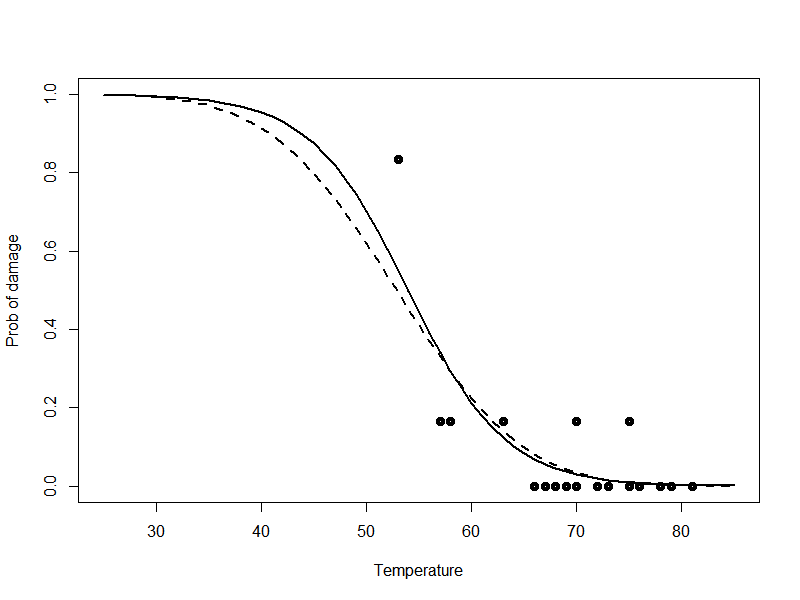
\includegraphics[width=1\textwidth,height=0.8\textheight]{logitplot1.png}
\end{center}
\end{frame}


\begin{frame}[containsverbatim]
\frametitle{Оценка качества биномиальной регрессии}
\begin{defn}
$$D\sim \chi^2(n-l)$$
где $n$ - количество наблюдений, $l$ - количество предикторов
\end{defn}
\begin{exmpr}
\begin{verbatim}
# для модели биномиальной регрессии
> pchisq(deviance(logitmod),df.residual(logitmod),lower=F)
[1] 0.7164099 
# для "нулевой" модели
> pchisq(38.9,22,lower=F)
[1] 0.01448877
\end{verbatim}
\end{exmpr}
\end{frame}


\begin{frame}[containsverbatim]
\frametitle{Оценка качества биномиальной регрессии}
\begin{defn}[Аналог статистики $R^2$]
$$R^2=\frac{1-exp((D-D_{null})/n)}{1-exp(-D_{null}/n)}$$
$n$ - общее количество наблюдений
\end{defn}
\begin{exmpr}
\begin{verbatim}
> modl<-glm(cbind(dead,alive)~conc,family=binomial,bliss)
> (1-exp((modl$dev-modl$null)/150))/(1-exp(-modl$null/150))
[1] 0.9953178
\end{verbatim}
\end{exmpr}
\end{frame}


\begin{frame}[containsverbatim]
\frametitle{Сравнение link function биномиальной регресси}
\begin{exmpr}
\begin{verbatim}
> modl<glm(cbind(dead,alive)~conc,family=binomial,
data=bliss)
> modp<glm(cbind(dead,alive)~conc,
family=binomial(link=probit),data=bliss)
> modc<-glm(cbind(dead,alive)~conc,
family=binomial(link=cloglog),data=bliss)
> x<-seq(-2,8,0.2)
> pl<-ilogit(modl$coef[1]+modl$coef[2]*x)
> pp<-pnorm(modl$coef[1]+modl$coef[2]*x)
> pc<-1-exp(-exp(modl$coef[1]+modl$coef[2]*x))
> plot(x,pl,type="l",ylab="Probability",xlab="Dose",lwd=2)
> lines(x,pp,lty=2,lwd=2)
> lines(x,pc,lty=6,lwd=2)
\end{verbatim}
\end{exmpr}

\end{frame}

\begin{frame}
\frametitle{Сравнение link function биномиальной регрессии}
\begin{center}
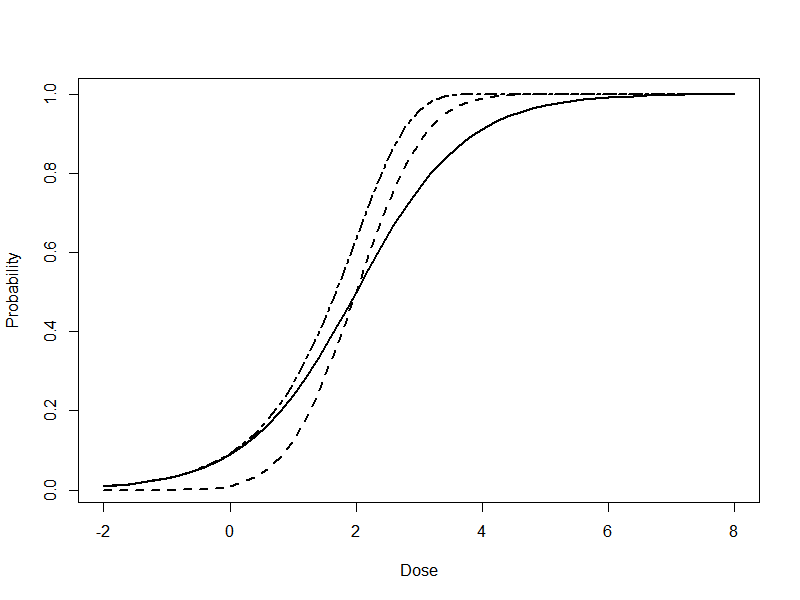
\includegraphics[width=1\textwidth,height=0.8\textheight]{linkplot1.png}
\end{center}
\end{frame}


\begin{frame}[containsverbatim]
\frametitle{Проблема сходимости в биномиальной регрессии}
\begin{exmpr}
\begin{verbatim}
> modl<-glm(orientation~estrogen+androgen,hormone,
family=binomial)
Warning messages:
1: glm.fit: algorithm did not converge 
2: glm.fit: fitted probabilities numerically 0 or 1
occurred
\end{verbatim}
\end{exmpr}

\end{frame}


\begin{frame}[containsverbatim]
\frametitle{Проблема сходимости в биномиальной регрессии}
\begin{exmpr}
\begin{verbatim}
> summary(modl)
Deviance Residuals: 
       Min          1Q      Median          3Q         Max  
-2.759e-05  -2.100e-08  -2.100e-08   2.100e-08   3.380e-05  
Coefficients:
             Estimate Std. Error z value Pr(>|z|)
(Intercept)    -84.49  136095.03  -0.001    1.000
estrogen       -90.22   75910.98  -0.001    0.999
androgen       100.91   92755.62   0.001    0.999
(Dispersion parameter for binomial family taken to be 1)
    Null deviance: 3.5426e+01  on 25  degrees of freedom
Residual deviance: 2.3229e-09  on 23  degrees of freedom
AIC: 6
Number of Fisher Scoring iterations: 25
\end{verbatim}
\end{exmpr}

\end{frame}

\begin{frame}[containsverbatim]
\frametitle{Проблема сходимости в биномиальной регрессии}
\begin{exmpr}
\begin{verbatim}
> plot(estrogen~androgen,data=hormone,
pch=as.character(orientation))
> abline(-84.5/90.2,100.9/90.2)
\end{verbatim}
\end{exmpr}
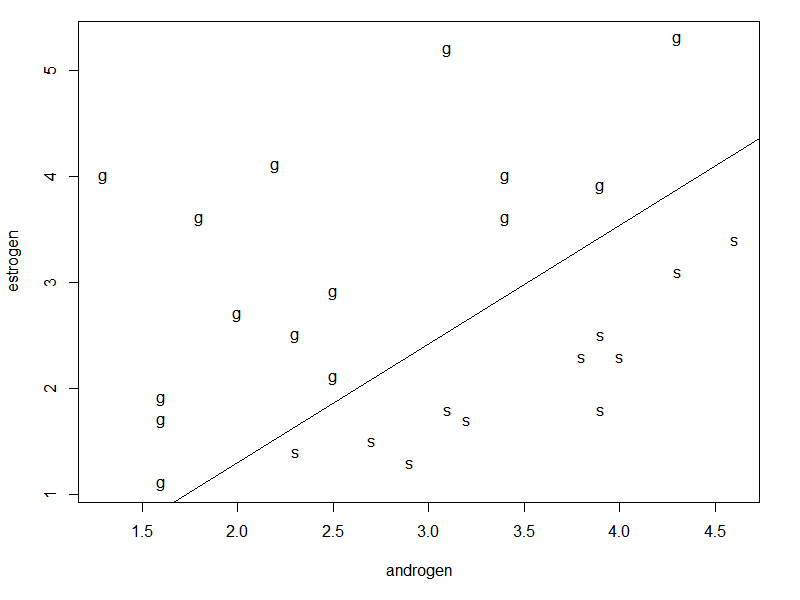
\includegraphics[width=1\textwidth,height=0.6\textheight]{logitplot2.png}
\end{frame}


\begin{frame}
\frametitle{Пуассоновская регрессия}
\begin{defn}
$$P(Y=y)=\frac{e^{-\mu}\mu^y}{y!}$$
Причины появления распределения Пуассона:\\
1) Вероятность успеха мала, а число случаев достаточно большое. Например, наличие редкой формы рака.\\
2) Вероятность события на некотором интервале времени пропорциональна его размеру и не зависит от появления других событий. Например, количество телефонных звонков.\\
3) Времена между событиями независимы и экспоненциально распределены.
Главное отличие от биномиального распределения - число успехов не ограничено.
\end{defn}
\end{frame}

\begin{frame}[containsverbatim]
\frametitle{Пуассоновская регрессия}
\begin{exmpr}
\begin{verbatim}
> modp<-glm(Species~Area+Elevation+Nearest+Scruz+
Adjacent,family=poisson,gala)
> summary(modp)  
Coefficients:
              Estimate Std. Error z value Pr(>|z|)    
(Intercept)  3.155e+00  5.175e-02  60.963  < 2e-16 ***
Area        -5.799e-04  2.627e-05 -22.074  < 2e-16 ***
Elevation    3.541e-03  8.741e-05  40.507  < 2e-16 ***
Nearest      8.826e-03  1.821e-03   4.846 1.26e-06 ***
Scruz       -5.709e-03  6.256e-04  -9.126  < 2e-16 ***
Adjacent    -6.630e-04  2.933e-05 -22.608  < 2e-16 ***
Signif.codes:0‘***’0.001‘**’0.01‘*’0.05‘.’0.1‘ ’1 
(Dispersion parameter for poisson family taken to be 1)
    Null deviance: 3510.73  on 29  degrees of freedom
Residual deviance:  716.85  on 24  degrees of freedom
AIC: 889.68
\end{verbatim}
\end{exmpr}
\end{frame}

\begin{frame}
\frametitle{Непараметрическая регрессия}
\begin{defn}
$$\hat{f}_{\lambda}(x)=\frac{1}{n\lambda}\sum_{j=1}^n{K\left(\frac{x-x_j}{\lambda}\right)Y_j}=\frac{1}{n}\sum_{j=1}^n{w_jY_j}$$
где $w_j=K\left(\frac{x-x_j}{\lambda}\right)/\lambda$ и $\int K(x)dx=1$. Функция $K$ называется ядром регрессии.
\end{defn}
\begin{defn}[Оценка Nadaraya-Watson]
$$f_{\lambda}(x)=\frac{\sum_{j=1}^n{w_jY_j}}{\sum_{j=1}^n{w_j}}$$
\end{defn}
\end{frame}

\begin{frame}[containsverbatim]
\frametitle{Непараметрическая регрессия}
\begin{exmpr}
\begin{verbatim}
> plot(waiting~eruptions,faithful,main="bandwidth=0.1")
> lines(ksmooth(faithful$eruptions,faithful$waiting,
"normal",0.1),lwd=2)
\end{verbatim}
\end{exmpr}
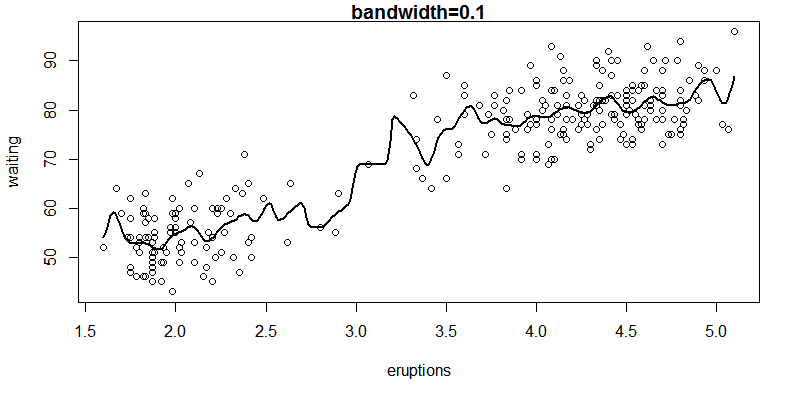
\includegraphics[width=1\textwidth,height=0.6\textheight]{ksmoothplot1.png}
\end{frame}

\begin{frame}[containsverbatim]
\frametitle{Непараметрическая регрессия}
\begin{exmpr}
\begin{verbatim}
> plot(waiting~eruptions,faithful,main="bandwidth=0.5")
> lines(ksmooth(faithful$eruptions,faithful$waiting,
"normal",0.5),lwd=2)
\end{verbatim}
\end{exmpr}
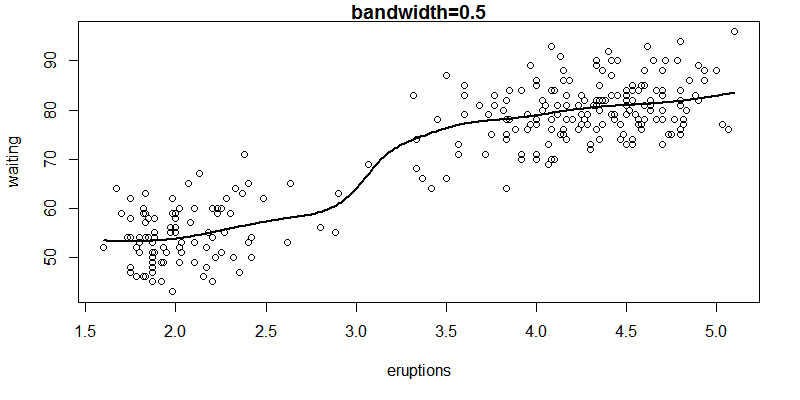
\includegraphics[width=1\textwidth,height=0.6\textheight]{ksmoothplot2.png}
\end{frame}

\begin{frame}[containsverbatim]
\frametitle{Непараметрическая регрессия}
\begin{exmpr}
\begin{verbatim}
> plot(waiting~eruptions,faithful,main="bandwidth=2")
> lines(ksmooth(faithful$eruptions,faithful$waiting,
"normal",2),lwd=2)
\end{verbatim}
\end{exmpr}
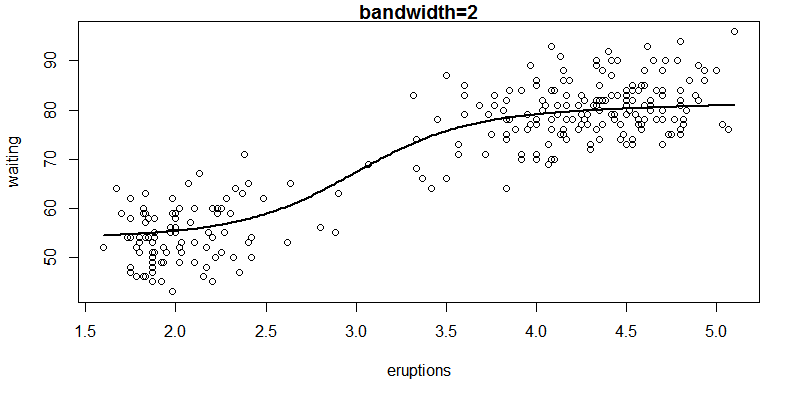
\includegraphics[width=1\textwidth,height=0.6\textheight]{ksmoothplot3.png}
\end{frame}

\begin{frame}
\frametitle{Аддитивные модели}
\begin{defn}
$$y=\beta_0+\sum_{j=1}^p{f_j(X_j)}+\epsilon$$
где $f_j$ - сглаживающие функции.
\end{defn}
\begin{defn}[Backfitting algorithm]
1) $\beta_0=\overline{y}$ и $f_j=0$\\
Повторять до сходимости:\\
2) $f_j=S(x_j,y-\beta(0)-\sum_{k\neq j}f_k)$\\
где $S$ - какая-нибудь сглаживающая функция.
\end{defn}
\end{frame}

\begin{frame}[containsverbatim]
\frametitle{Аддитивные модели}
\begin{exmpr}
\begin{verbatim}
> amgam<-gam(O3~lo(temp)+lo(ibh)+lo(ibt),data=ozone)
> summary(amgam)
Deviance Residuals:
     Min       1Q   Median       3Q      Max 
-13.1146  -2.3624  -0.2092   2.1732  12.4447 
(Dispersion Parameter for gaussian family taken to be 18.6638)
    Null Deviance: 21115.41 on 329 degrees of freedom
Residual Deviance: 5935.096 on 318.0005 degrees of freedom
AIC: 1916.049 
Number of Local Scoring Iterations: 2 
DF for Terms and F-values for Nonparametric Effects
            Df Npar Df Npar F     Pr(F)    
(Intercept)  1                             
lo(temp)     1     2.5 7.4550 0.0002456 ***
lo(ibh)      1     2.9 7.6205 8.243e-05 ***
lo(ibt)      1     2.7 7.8434 9.917e-05 ***
\end{verbatim}
\end{exmpr}
\end{frame}

\begin{frame}[containsverbatim]
\frametitle{Аддитивные модели}
\begin{exmpr}
\begin{verbatim}
> plot(amgam,residuals=T,se=T,pch="*")
\end{verbatim}
\end{exmpr}
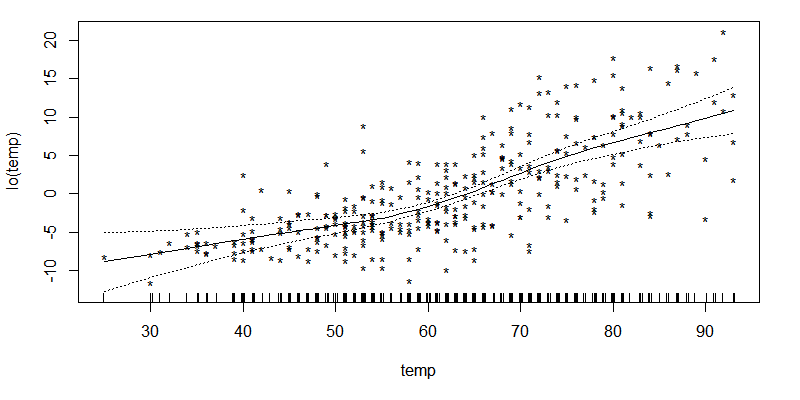
\includegraphics[width=1\textwidth,height=0.6\textheight]{gamplot1.png}
\end{frame}

\begin{frame}
\frametitle{Регуляризация}
\begin{defn}[Ридж регрессия]
$$J(\theta)=\frac{1}{2}(y-f(X\theta))^T(y-f(X\theta))+\frac{\lambda}{2}||\theta||_{L^2}$$
\end{defn}
\begin{defn}[Лассо регрессия]
$$J(\theta)=\frac{1}{2}(y-f(X\theta))^T(y-f(X\theta))+\frac{\lambda}{2}||\theta||_{L^1}$$
\end{defn}
\end{frame}

\begin{frame}[containsverbatim]
\frametitle{Регуляризация}
\begin{exmpr}
\begin{verbatim}
> library(penalized)
> data(nki70)
> lmr1 <- penalized(ER~DIAPH3+NUSAP1,data=nki70,lambda1=1)
# nonzero coefficients: 2
> lmr2 <- penalized(ER~DIAPH3+NUSAP1,data=nki70,lambda2=1)
> coefficients(lmr1)
(Intercept)      DIAPH3 
   1.457045   -1.587166
> coefficients(lmr2)
(Intercept)      DIAPH3      NUSAP1 
  1.4475712  -1.2150576  -0.2340205
\end{verbatim}
\end{exmpr}
\end{frame}

\begin{frame}[containsverbatim]
\frametitle{Изменение коэффициентов в лассо регрессии}
\begin{exmpr}
\begin{verbatim}
lmr1 <- penalized(ER~DIAPH3+NUSAP1, data=nki70,
lambda1=0,step=50)
plotpath(lmr1,lwd=2)
\end{verbatim}
\end{exmpr}
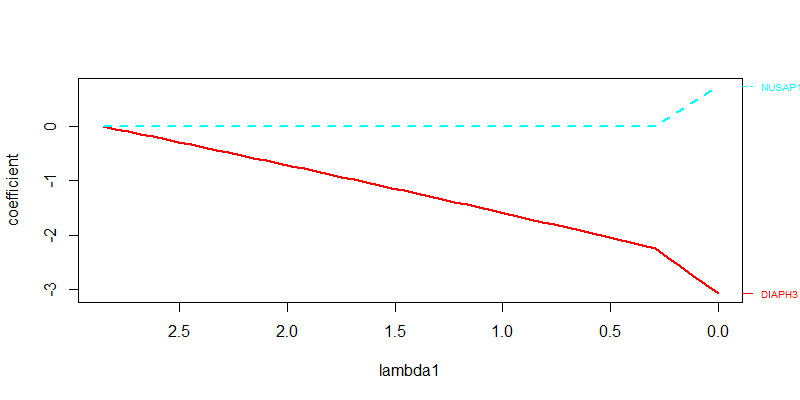
\includegraphics[width=1\textwidth,height=0.6\textheight]{penalizedplot1.png}
\end{frame}

\begin{frame}[containsverbatim]
\frametitle{Подбор оптимального параметра $\lambda_1$}
\begin{exmpr}
\begin{verbatim}
> profL1(ER~DIAPH3+NUSAP1, data=nki70,plot=T,trace=F)
> optL1(ER~DIAPH3+NUSAP1, data=nki70,trace=F)$lambda
[1] 0.5486795
\end{verbatim}
\end{exmpr}
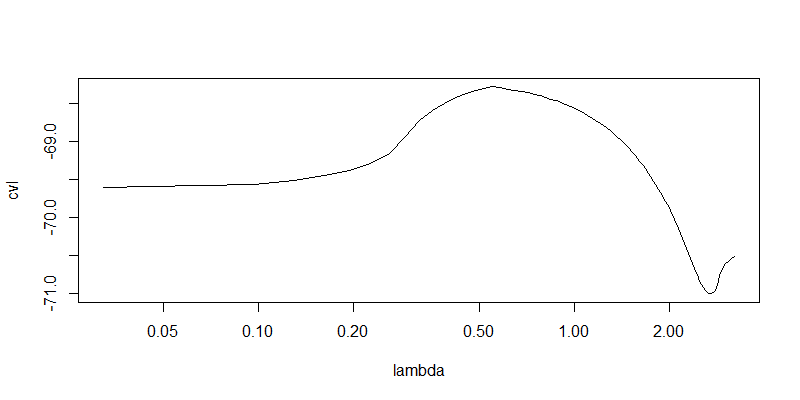
\includegraphics[width=1\textwidth,height=0.6\textheight]{penalizedplot2.png}
\end{frame}

\begin{frame}[containsverbatim]
\frametitle{Подбор оптимального параметра $\lambda_2$}
\begin{exmpr}
\begin{verbatim}
> profL2(ER~DIAPH3+NUSAP1,data=nki70,minlambda=0.01,
maxlambda=5,plot=T,trace=F)
> optL2(ER~DIAPH3+NUSAP1, data=nki70,trace=F)$lambda
[1] 0.6114319
\end{verbatim}
\end{exmpr}
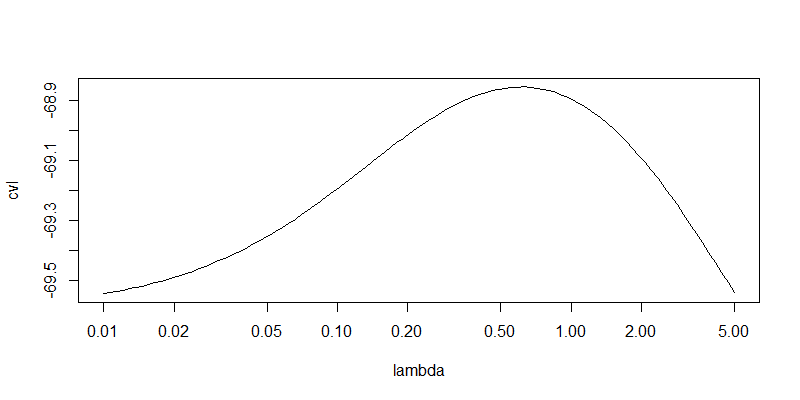
\includegraphics[width=1\textwidth,height=0.6\textheight]{penalizedplot3.png}
\end{frame}

\end{document}